\documentclass[11pt, oneside, a4paper]{article}

\usepackage{pdfpages}
\usepackage{fontspec}
\usepackage{titlesec}
\usepackage{xcolor}
\usepackage{graphicx}
\usepackage[colorlinks=true]{hyperref}
\usepackage[font={footnotesize,it}]{caption}
\usepackage{booktabs}
\usepackage{multirow}
\usepackage{tabularx}
\usepackage{apacite}
\usepackage{array}
\usepackage{colortbl}
\usepackage{fancyhdr}
\usepackage[hmargin=0.8in,vmargin=1in]{geometry}

\newfontfamily\headingfont{Titillium Web SemiBold}
\newfontfamily\subheadingfont{Titillium Web}
\newfontfamily\authorfont{Roboto Slab}

\titleformat{\section}{\headingfont{}\LARGE\color{cyan}}{\thesection}{1em}{}
\titleformat{\subsection}{\subheadingfont{}\Large}{\thesubsection}{1em}{}
\titleformat{\subsubsection}{\subheadingfont{}\large\itshape}{\thesubsubsection}{1em}{}

\setmainfont{Cambria}

\graphicspath{{./Figures/}}

\pagestyle{fancy}
\fancyhf{}
\fancyhead[L]{\leftmark}
\fancyhead[R]{TensorOverflow}
\fancyfoot[C]{\thepage}

\setlength{\parindent}{0pt}

\begin{document}
\begin{titlepage}
    \begin{center}
        \vspace*{5cm}
 
        {\LARGE\headingfont{Face Encryption}}

        \vspace{2cm}
        SDS3386 Data Science Lab
        
        \vspace{0.5cm}
        Fall 2022


        \vspace{1.5cm}
        \textbf{Team TensorOverflow}

        \vspace{1.5cm}
        \begin{tabular}{rl}
            Xiang Li & 300056427 \\
            Jiaxun Gao & 300063462 \\
            Bowen Zeng & 300115382  \\
        \end{tabular}
 
        \vfill
             
        Course Coordinator: Tanya Schmah\\
        
        \vspace{0.5cm}
        November 30, 2022

        \vspace{1cm}
        University of Ottawa

        \vspace{0.8cm}
      
        \includegraphics[width=0.2\textwidth]{uOttawa.png}
             

        \date{}
             
    \end{center}
 \end{titlepage}

{\hypersetup{hidelinks}
    \tableofcontents
    \newpage
    %\listoffigures
    %\newpage
    %\listoftables
    %\newpage
}

    \hypersetup{
        linkcolor = blue,
        bookmarksnumbered=true
    }

    \section{Introduction}

Recent research \cite{6227909} has verified that there are recognized privacy dangers related to the massive amounts of user-generated information published on public social media platforms. Internet behemoths like Google and Facebook have been secretly mining this data without the users' awareness or permission \cite{10.1093/idpl/ipw026}. When personal photos of people's faces are uploaded, this creates a severe privacy risk for those depicted. Companies may use these photographs to train machine learning algorithms, which could compromise users' personal information. \textbf{What measures can we take to ensure that individuals' privacy is maintained when exchanging photographs of their faces?}

We present a method that safeguards users' privacy when exchanging facial images by utilizing adversarial attacks and facial recognition algorithms. To accomplish this, we first use a facial recognition model to identify individuals in a picture, and then we encrypt their likenesses using noise produced by an adversarial attacking model. While the resulting image may have high visual similarities between human eyes, facial recognition software will fail to re-identify the right person in it. Such a facial encryption process can help people feel more comfortable sharing photographs online while maintaining their privacy.



    \section{Dataset}

\subsection{CelebA} \label{sec:CelebA}

CelebA is a large-scale face attributes dataset with more than 200K celebrity images, each with 40 attribute annotations. The images in this dataset cover large pose variations and background clutter. CelebA has large diversities, large quantities, and rich annotations, including \textbf{5,000 celebrity identities}, \textbf{202,599 face images}, and \textbf{40 binary attributes} annotations per image. The dataset can be employed as the training and test sets for the following computer vision tasks: face attribute recognition, face detection, landmark (or facial part) localization, and face editing/synthesis.

% insert the image of the dataset
\begin{figure}[h]
\centering
\includegraphics[width=0.5\textwidth]{CelebA_stat.png}
\caption{CelebA dataset distribution}
\label{fig:CelebA_stat}
\end{figure}

\begin{figure}[htbp]
    \centering
    \begin{subfigure}{0.4\textwidth}
        \centering
        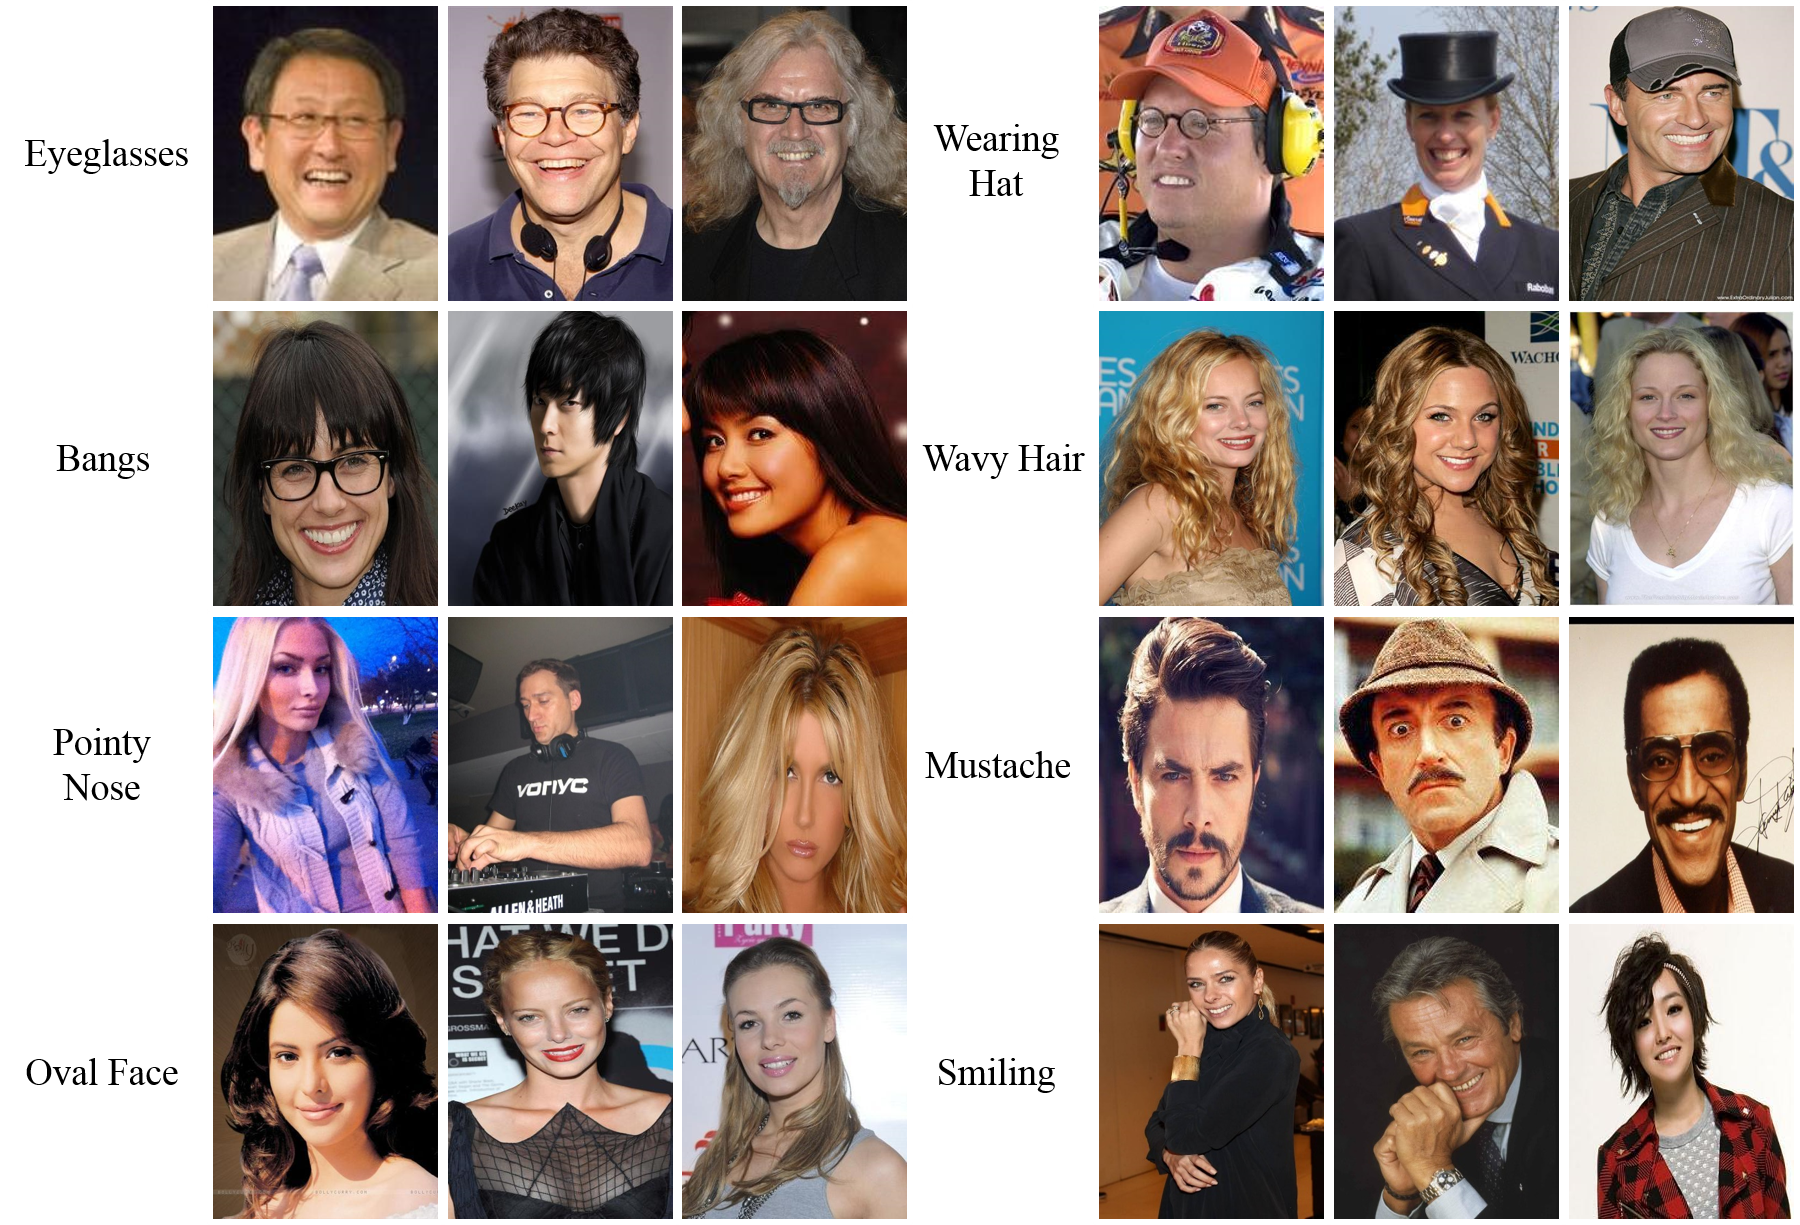
\includegraphics[width=1\textwidth]{CelebA.png}
        \caption{CelebA dataset covers large pose variations}
    \end{subfigure}
    \qquad
    \begin{subfigure}{0.4\textwidth}
        \centering
        \includegraphics[width=1\textwidth]{CelebA_usage.png}
        \caption{CelebA in face recognition}
    \end{subfigure}
    \caption{An excerpt from CelebA dataset}
    \label{fig:CelebA}
\end{figure}

In this project, we utilized a subset of CelebA as the face recognition model's dataset. The dataset includes 5696 images of 307 different people, with 4429 images used for training and 1267 images used for testing.

\subsection{Private Dataset}

For a better presentation, we also constructed a private dataset consisting 121 images of all team members. The photos were cropped from 3 videos, which were uniformly sampled to 40 frames each to vary the facial expression. In each frame, the face image is detected by package Mediapipe and then stored in the local device. \footnote{This process is done in Data\_generation.ipynb.ipynb.}

The private dataset and CelebA dataset together form the training and testing dataset of our face recognition model.

    \section{Methodology}

\subsection{Adversarial Attacks}

% explain what is adversarial attacking

Adversarial attacking is a technique that can be used to fool machine learning models. It is a type of attack that aims to change the input data in a way that the model will misclassify it. The adversarial attacking technique is based on the fact that machine learning models are vulnerable to small perturbations in the input data. The perturbations are usually imperceptible to the human eye, but they can cause the model to misclassify the input data.

Adversarial examples are hard to defend against because it is difficult to construct a theoretical model of the adversarial example crafting process. Adversarial examples are solutions to an optimization problem that is non-linear and non-convex for many ML models, including neural networks. Because we don't have good theoretical tools for describing the solutions to these complicated optimization problems, it is very hard to make any kind of theoretical argument that a defense will rule out a set of adversarial examples.

\begin{figure}[h]
    \centering
    \includegraphics[width=0.8\textwidth]{adversarial_attack.png}
    \caption{An adversarial input, overlaid on a typical image, can cause a classifier to miscategorize a panda as a gibbon.}
    \label{fig:adversarial_attack}
\end{figure}
    

Another reason is they require machine learning models to produce good outputs for every possible input. Most of the time, machine learning models work very well but only work on a very small amount of all the many possible inputs they might encounter. \cite{adversarial_2020}


\subsection{Backbone Model: ResNet-18}

% explain what is ResNet-18

ResNet-18 is a convolutional neural network (CNN) that is used as a backbone model in this project. The architecture can be illustrated as figure \ref{fig:resnet18} \cite{ResNet-18}.
It is a 18-layer deep neural network that is trained on the ImageNet dataset. The ImageNet dataset is a large dataset that contains 1.2 million images with 1000 classes. The ResNet-18 model is trained on the ImageNet dataset to classify the images into 1000 classes.

% insert the ResNet-18 picture

\begin{figure}[h]
\centering
\includegraphics[width=1\textwidth]{ResNet18.png}
\caption{ResNet-18 Architecture}
\label{fig:resnet18}
\end{figure}


    \section{Data Wrangling}


\subsection{Faces extraction from recorded video}

After capturing three videos, OpenCV2 is used to sample 40 frames from each video. The faces are then rotated 180 degrees to accommodate package mediapipe's face detection model. Then, we crop the faces from the frames using the centre of the bounding box's coordinates. The faces are then saved in a folder named \verb|private_dataset| and added to \verb|CelebA_HQ_facial_identity_dataset|.

This process is done in \verb|Data_generation.ipynb.ipynb|.


\subsection{Associate id with name}

After downloading the CelebA dataset from the official website, we utilise CelebA-HQ-to-CelebA-mapping.txt to generate a map \verb|hq_A_mapping| from an id to the image file name, such as \verb|5: 000615.jpg|.
Then, we use list\_identity\_celeba.txt to generate the second map \verb|id_name_mapping| from a file name to its corresponding identity's name, for instance: \verb|000615.jpg: Martha Hunt|.

The benefit of this process is that we can now use the id to determine an identity's name. By example, we may use the following code: \verb|id_name_mapping[hq_A_mapping['5']]| to determine the name of the individual with id = 5.

This process is done in \verb|Preprocessing.ipynb|.

\subsection{Transforming the dataset}

We resized the images to 224x224 because their original size was too large for our model, which could cause performance issues. After that, we augment the tensor by giving it a random horizontal flip as part of the transformation.

This process is a part of \verb|simple_model.ipynb|.

    \newpage

    \bibliographystyle{apacite} % We choose the "plain" reference style
    \bibliography{references}


\end{document}
